\documentclass{article}
\usepackage[utf8]{inputenc}
\usepackage{graphicx}
	\DeclareGraphicsExtensions{.png, .jpeg}
\usepackage{caption}
\usepackage{csvsimple}
\usepackage[top=1in, bottom=1in, left=1in, right=1in]{geometry}

\title{Database Design and Implementation \\ HW 04}
\author{\underline{Team 08}\\Henriod, Terence\\Santoyo, Jorge\\Singh, Raja}
\date{\today}

\begin{document}

\clearpage
\maketitle
\thispagestyle{empty} % removes the page number from the title page

\begin{abstract}
An introductory assignment to become familiarized with writing queries using the SQL SELECT statement.
\end{abstract}

\newpage
\section{Assignment Background}
The objectives for this assignment are to:
\begin{enumerate}
  \item Learn how to write simple, 1 table SQL queries;
  \item Become more familiar with the CutGlass job costing database; and
  \item Learn about each component of the SQL SELECT statement.
\end{enumerate}
Each of the questions in this homework assignment requires you to create a SELECT statement to satisfy the request. There are 15 questions that should produce 15 SELECT queries for this assignment. None of the questions require that you join tables to create the answer. 

\newpage
\section{SQL Query Problems}
\begin{enumerate}
  \item %\\
  \textit{Solution}:
  \begin{verbatim}
       SELECT ClientID 'Clientid',
          ClientName,
          ClientCity,
          ClientState,
          ClientZip,
          Phone  'ClientPhone'
       FROM Client
       WHERE ClientCity = 'Reno';
  \end{verbatim}

  \begin{figure}[h!]
    \centering
    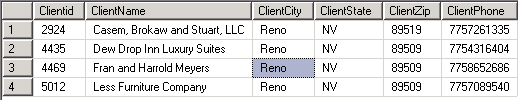
\includegraphics[width=.8\linewidth]{QueryResults/HW04_Problem01_query}
    \caption{The solution to problem 1.}
    \label{fig:HW04_Problem01}
  \end{figure}

  \newpage
  \item %\\
  \textit{Solution}:
  \begin{verbatim}
      SELECT  ClientID 'ClientId',
          ClientName 'Client Name ',
          ClientCity 'Client Billing City ',
          ClientState 'Client Billing State',
          ClientZip 'Client Billing Zip',
            STUFF(STUFF(STUFF(Phone,1,0,'('),6,0,') '),11,0,'-') as 'Client Billing Phone'
       FROM Client
       WHERE ClientCity = 'Reno'
       ORDER BY ClientZip;
  \end{verbatim}

  \begin{figure}[h!]
    \centering
    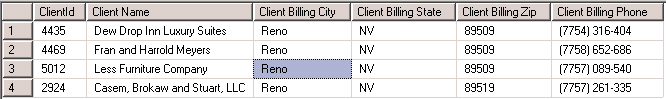
\includegraphics[width=.8\linewidth]{QueryResults/HW04_Problem02_query}
    \caption{The solution to problem 2.}
    \label{fig:HW04_Problem02}
  \end{figure}

  \newpage
  \item %List the JobID, JobName, DateProposed, DateAccepted, EmpManagerID, and PrimaryJobID from the Job table. Create a message in a column called``JobCompletedMessage" that says ``Job Not Finished" if the JobComplete flag is 0, and says ``Job Finished" if the JobComplete flag is $1$. If the DateAccepted is NULL, then put a message in the column that says ``Not Accepted". Sort the result table by DateProposed so that the most recent date is the first row in the result table.\\
  %Hints: Use the CASE statement to generated the JobCompletedMessage. Use the ISNULL function to generate the ``Not Accepted" message in the DateAccepted field. Use the CONVERT function to change the date from a date field to a to a varchar field.\\

  \textit{Solution}:
  \begin{verbatim}
       SELECT
          JobID 'Job ID'
        , JobName 'Job Name'
        , DateProposed  'Date Proposed'
        , ISNULL(CONVERT(VARCHAR, DateAccepted, 120), 'Not Accepted') 'Date Accepted'
        , EmpManagerID  'Employee Manager ID'
        , PrimaryJobID  'Primary Job ID'
        , CASE
          WHEN JobCompleted = 1
            THEN 'Job Finished'
          ELSE
            'Job Not Finished'
          END 'Job Completed Message'
      FROM
        Job
      ORDER BY
        DateProposed DESC
      ;
  \end{verbatim}

  \begin{figure}[h!]
    \centering
    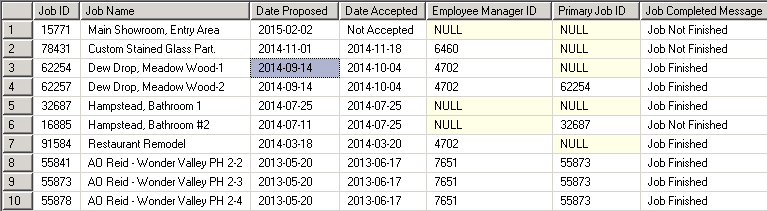
\includegraphics[width=.95\linewidth]{QueryResults/HW04_Problem03_query}
    \caption{The solution to problem 3.}
    \label{fig:HW04_Problem03_query}
  \end{figure}

  \newpage
  \item %\\
  \textit{Solution}:
  \begin{verbatim}
      SELECT JobID,
           TaskID,
           DateStarted,
           EstMaterialCost/SquareFeet 'EstMaterialCostperSqft',
           EstLaborCost/SquareFeet 'EstLaborCostperSqft',
           EstLaborCost/EstHours 'EstLaborCostperHr'
      FROM JobTask
      WHERE DATEDIFF(YYYY,  DateCompleted, GETDATE()) = 2
      ORDER BY TaskID;
  \end{verbatim}

  \begin{figure}[h!]
    \centering
    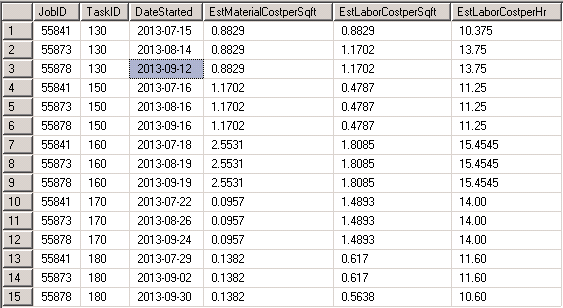
\includegraphics[width=.8\linewidth]{QueryResults/HW04_Problem04_query}
    \caption{The solution to problem 4.}
    \label{fig:HW04_Problem04}
  \end{figure}
  
  \newpage
  \item %\\
  \textit{Solution}:
  \begin{verbatim}
      SELECT 
        ROUND(AVG(EstMaterialCost/SquareFeet),2) 'Average EstMaterialCostPerSqFt',
        ROUND(MAX(EstMaterialCost/SquareFeet),2) 'Largest EstMaterialCostPerSqFt',
        ROUND(MIN(EstMaterialCost/SquareFeet),2) 'Smallest EstMaterialCostPerSqFt',
        ROUND(AVG(EstLaborCost/SquareFeet),2) 'Average EstLaborCostPerSqFt',
        ROUND(MAX(EstLaborCost/SquareFeet),2) 'Largest EstLaborCostPerSqFt',
        ROUND(MIN(EstLaborCost/SquareFeet),2) 'Smallest EstLaborCostPerSqFt'  
      FROM 
        JobTask
      WHERE
        DateCompleted is not NULL AND
        DATEDIFF(YEAR, DateCompleted, GETDATE()) = 2;
  \end{verbatim}

  \begin{figure}[h!]
    \centering
    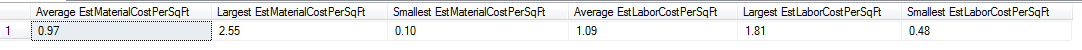
\includegraphics[width=.95\linewidth]{QueryResults/HW04_Problem05_query}
    \caption{The solution to problem 5.}
    \label{fig:HW04_Problem05}
  \end{figure}
  
  \newpage
  \item %Most tasks on most jobs are finished within $3$ days of the start date for the task. List only those tasks in the JobTask table that took more than $3$ days to complete. For any task that took over $5$ days to complete, put a message in a created column that says ``Late Completion – Investigate". Sort the output by taskID within JobID.\\

  \textit{Solution}:
  \begin{verbatim}
      /** Assumption: if a job is not currently complete, it makes
       * no sense to compute a completion time yet - let the result
       * be NULL. Also, don't consider incomplete jobs.
       */
      SELECT
            JobID 'Job ID'
          , TaskID 'TaskID'
          , DateStarted 'Date Started'
          , DateCompleted 'Date Completed'
          , DATEDIFF(DAY, DateStarted, DateCompleted)
          , CASE
            WHEN DATEDIFF(DAY, DateStarted, DateCompleted) > 5
              THEN 'Late Completion - Investigate'
            ELSE
              '' -- No message for typical completion times was specified
            END 'Message'
      FROM
        JobTask
      WHERE
            DateCompleted IS NOT NULL
        AND DATEDIFF(DAY, DateStarted, DateCompleted) > 3
      ORDER BY
          JobID
        , TaskID
      ;
  \end{verbatim}

  \begin{figure}[h!]
    \centering
    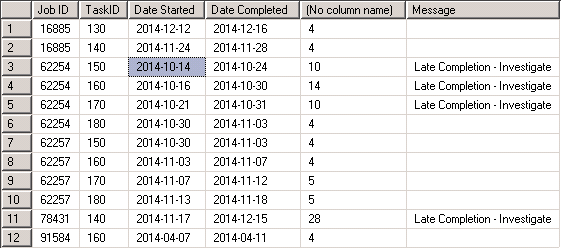
\includegraphics[width=.6\linewidth]{QueryResults/HW04_Problem06_query}
    \caption{The solution to problem 6.}
    \label{fig:HW04_Problem06_query}
  \end{figure}

  \newpage
  \item %\\
  \textit{Solution}:
  \begin{verbatim}
      SELECT 
        JobID,
        TaskID,
        Count(*) 'NumberOfTimeCards',
        SUM(HoursWorked) 'TotalHoursWorked'
      FROM 
        TimeSheet
      GROUP BY
        JobID,TaskID
      ORDER BY
        JobID,TaskID
  \end{verbatim}

  \begin{figure}[h!]
    \centering
    \begin{minipage}{.5\textwidth}
      \centering
      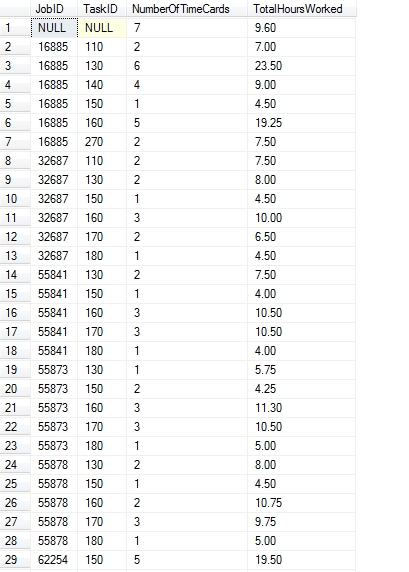
\includegraphics[width=.8\linewidth]{QueryResults/HW04_Problem07a_query}
      \caption{The solution to problem 7 (the first half).}
      \label{fig:HW04_Problem07a}
    \end{minipage}%
    \begin{minipage}{.5\textwidth}
      \centering
      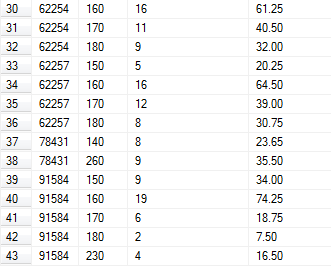
\includegraphics[width=.7\linewidth]{QueryResults/HW04_Problem07b_query}
      \caption{The solution to problem 7 (the second half).}
      \label{fig:HW04_Problem07b}
    \end{minipage}
  \end{figure}

  \newpage
  \item %\\
  \textit{Solution}:
  \begin{verbatim}
      SELECT 
        ISNULL(CONVERT(VARCHAR, JobID, 120),'No JobID') 'JobID',
        ISNULL(CONVERT(VARCHAR, TaskID, 120),'No TaskID') 'TaskID',
        COUNT(*)  'NumberOfTimeCards',
        SUM(HoursWorked) 'TotalHoursWorked'
      FROM 
        TimeSheet
      GROUP BY
        JobID,TaskID
      HAVING 
        COUNT(*) > 5
      ORDER BY
        JobID ,TaskID
  \end{verbatim}

  \begin{figure}[h!]
    \centering
    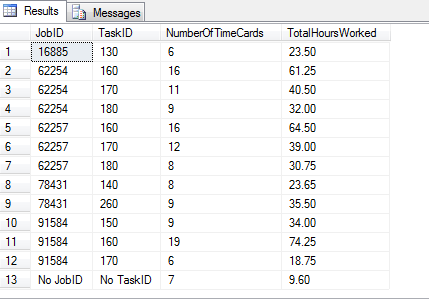
\includegraphics[width=.5\linewidth]{QueryResults/HW04_Problem08_query}
    \caption{The solution to problem 8.}
    \label{fig:HW04_Problem08}
  \end{figure}

  \newpage
  \item %Most of the employee time sheets in the TimeSheet table are for activities that are assigned directly to a task on a job. However, CutGlass occasionally has employee time sheets (time that they pay) for activities that are not directly assigned to a task on a job. When an employee’s time sheet is assigned to a task on a job, then the ``activity" column is null. For other activities, the activity column has a value. The goal of this query is to display summarized information about employee time sheets that do not have a null value in the activity column. This query should help you learn about how to display data that is not null. Display the EmpID, the total number of hours worked, and a count of the time sheets for that situation.\\

  \textit{Solution}:
  \begin{verbatim}
      SELECT
          EmpID 'Employee ID'
        , SUM(HoursWorked) 'Total Hours Not Assigned To Job'
        , COUNT(*)'Time Sheets Not Assigned To Job'
      FROM
        TimeSheet
      WHERE
        Activity IS NOT NULL
      GROUP BY
        EmpID
      ;
  \end{verbatim}

  \begin{figure}[h!]
    \centering
    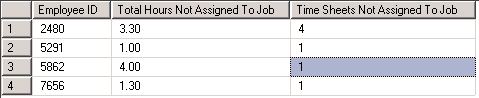
\includegraphics[width=.5\linewidth]{QueryResults/HW04_Problem09_query}
    \caption{The solution to problem 9.}
    \label{fig:HW04_Problem09_query}
  \end{figure}

  \newpage
  \item %\\

  \textit{Solution}:
  \begin{verbatim}
      SELECT EmpID,
             HourlyPayRate
      FROM EmployeePay
      WHERE EmpID = 6460 AND( ((convert(date, 'June 18, 2013')) BETWEEN DateStartPay AND DateEnd) OR ((convert (date, 'June 18, 2013') > DateStartPay AND DateEnd IS NULL)));
  \end{verbatim}

  \begin{figure}[h!]
    \centering
    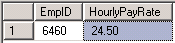
\includegraphics[width=.2\linewidth]{QueryResults/HW04_Problem10_query}
    \caption{The solution to problem 10.}
    \label{fig:HW04_Problem10}
  \end{figure}

  \newpage
  \item %\\

  \textit{Solution}:
  \begin{verbatim}
      SELECT 
        DISTINCT YEAR(DatePurchased) 'Purchase Year',
        COUNT(*) 'Number of Purchase Orders',
        SUM(Quantity) 'Total Quantity Purchased',
        SUM(Quantity * CostPerUOM) 'Total Amount Purchased'
      FROM 
        MaterialPurchased
      GROUP BY
        YEAR(DatePurchased);
  \end{verbatim}

  \begin{figure}[h!]
    \centering
    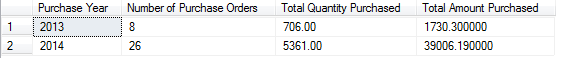
\includegraphics[width=.8\linewidth]{QueryResults/HW04_Problem11_query}
    \caption{The solution to problem 11.}
    \label{fig:HW04_Problem11}
  \end{figure}

  \newpage
  \item %Summarize the MaterialAssigned in the MaterialAssigned table by JobID and the year of the dateassigned. Display the year of the dateassigned, the jobID and the sum of the quantity of the material assigned. Sort the result table by jobID within year of date assigned.\\

  \textit{Solution}:
  \begin{verbatim}
      SELECT
          YEAR(DateAssigned) 'Assigned Year'
        , JobID 'JobID'
        , SUM(Quantity) 'Total Material Quantity Assigned'
      FROM
        MaterialAssigned
      GROUP BY
          YEAR(DateAssigned)
        , JobID
      ORDER BY
          YEAR(DateAssigned)
        , JobID
      ;
  \end{verbatim}

  \begin{figure}[h!]
    \centering
    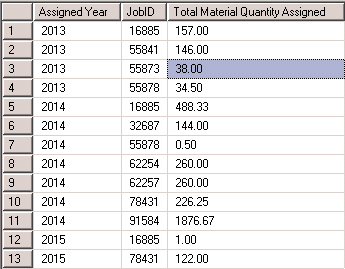
\includegraphics[width=.5\linewidth]{QueryResults/HW04_Problem12_query}
    \caption{The solution to problem 12.}
    \label{fig:HW04_Problem12_query}
  \end{figure}

  \newpage
  \item %\\
  \textit{Solution}:
  \begin{verbatim}
      SELECT
        ClientName
      FROM
        Client
      WHERE 
        ClientID not in (
          SELECT 
            ClientID 
          FROM 
            JOB
        )
      ORDER BY
        ClientName;
  \end{verbatim}

  \begin{figure}[h!]
    \centering
    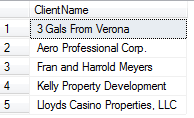
\includegraphics[width=.3\linewidth]{QueryResults/HW04_Problem13_query}
    \caption{The solution to problem 13.}
    \label{fig:HW04_Problem13}
  \end{figure}

  \newpage
  \item %\\
  \textit{Solution}:
  \begin{verbatim}
      SELECT ClientName,
           ClientZip,
           Email
      From Client
      WHERE ClientID In (
          SELECT ClientID
          FROM Job
          WHERE 2014 = DATEPART(YEAR, DateAccepted))
      ORDER BY ClientName;
  \end{verbatim}

  \begin{figure}[h!]
    \centering
    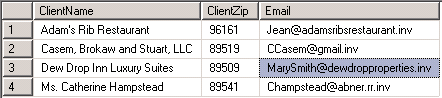
\includegraphics[width=.5\linewidth]{QueryResults/HW04_Problem14_query}
    \caption{The solution to problem 14.}
    \label{fig:HW04_Problem14}
  \end{figure}

  \newpage
  \item %What are the names of the employees who have not worked as a manager for a job in the Job table? Hint: this query requires the use of a non-correlated sub-query, and you need to consider that some of the empmanagerID’s in the Job table are null values.\\

  \textit{Solution}:
  \begin{verbatim}
      SELECT
        (LastName + ', ' + SUBSTRING(FirstName, 1, 1) + '.') 'Employee Name'
      FROM
        Employee
      WHERE
        EmpID NOT IN (
          SELECT
            EmpManagerID
          FROM
            Job
          WHERE
            EmpManagerID IS NOT NULL
        )
      ORDER BY
        LastName
      ;
  \end{verbatim}

  \begin{figure}[h!]
    \centering
    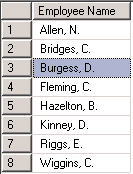
\includegraphics[width=.2\linewidth]{QueryResults/HW04_Problem15_query}
    \caption{The solution to problem 15.}
    \label{fig:HW04_Problem15_query}
  \end{figure}
\end{enumerate}

\end{document}
